%!TEX root = ../report.tex

\section{Network Layer}
The network layer serves the following functions:
\begin{itemize}
  \item IP protocol for addressing, datagram format and packet handling conventions
  \item Routing protocols for path selection
  \item ICMP protocol for error reporting and router signaling
\end{itemize}

\subsection{Internet Protocol}
\begin{figure}[H]
  \centering
  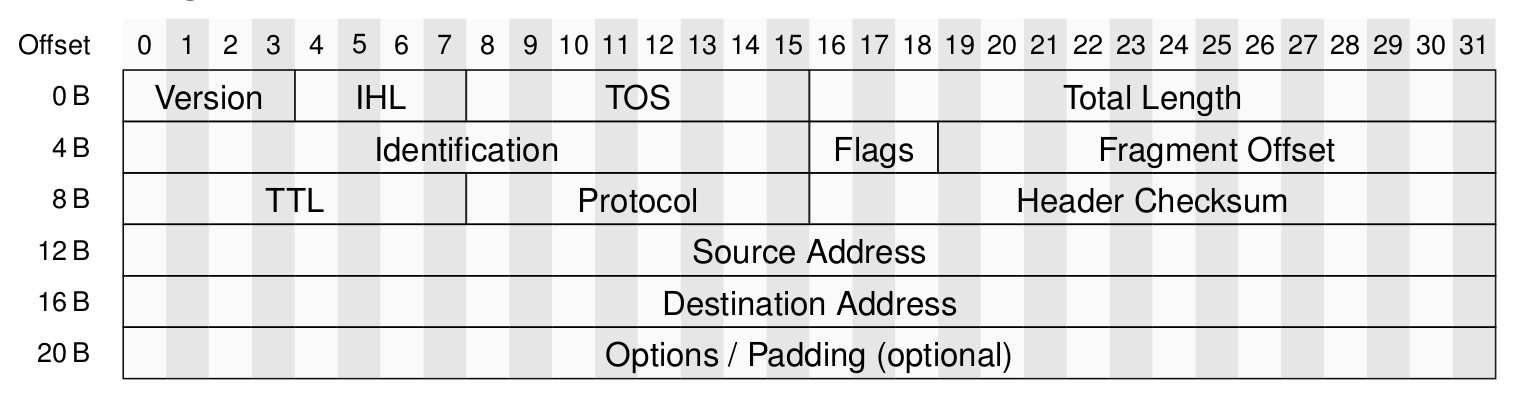
\includegraphics[width=.8\textwidth]{figures/ipv4_datagram.png}
  \caption{IPv4 Datagram}\label{fig:ipv4_datagram}
\end{figure}

\subsubsection*{IPv4 Addressing}
IPv4 addresses are 32-bit identifiers for every host and router interface where interfaces represent the connection between host/router and physical link.

Subnets are device interfaces with the same subnet part of the IP address which can physically reach each other without intervening router.

Splitting the IP address into network and host part is done in the following way (for the address 192.168.128.1/17):
\begin{figure}[H]
  \centering
  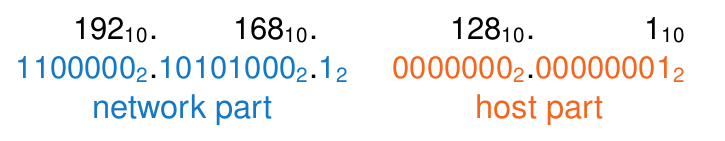
\includegraphics[width=.6\textwidth]{figures/ip_split.png}
\end{figure}

From 1982 to 1993, IP addresses were classfully divided as shown in Figure~\ref{fig:classful_ips}.
\begin{figure}[h]
  \centering
  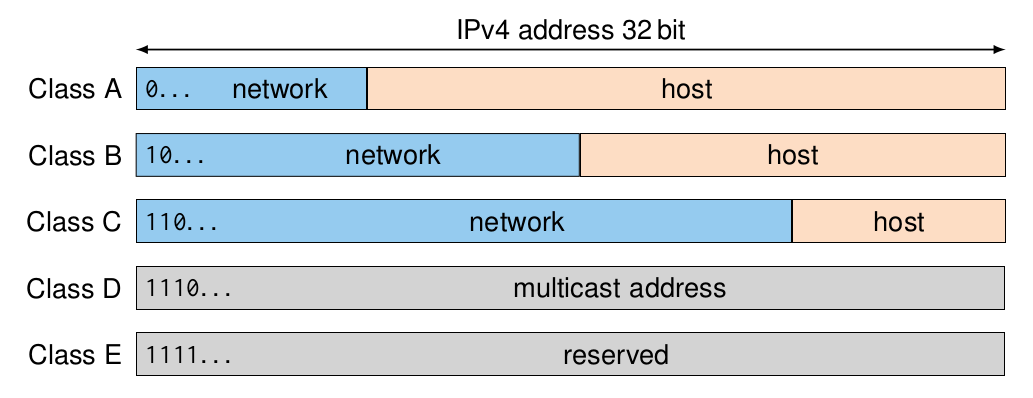
\includegraphics[width=.8\textwidth]{figures/classful_ip.png}
  \caption{Classful IPs}\label{fig:classful_ips}
\end{figure}
In 1993, Classless Inter-Domain Routing (CIDR) was introduced which allowed arbitrary subnet length.
To route packets, prefix matching is used which checks which entry in the routing table fits best for the incoming packet's network prefix.

\subsection{ICMP}
The Internet Control Message Protocol (ICMP) are located above IP but can be considered as part of the IP layer.
It is used for communicating error messages and other attention requiring conditions for IP and TCP or UDP\@.
Two classes of ICMP messages are possible:
\begin{enumerate}
  \item Query messages: only kind that generates other ICMP messages
  \item Error messages: contain IP header and first 8 bytes (today as much as possible up to 572 bytes) of datagram that caused the ICMP message which allows the receiver to put it into context
\end{enumerate}
The structure of an ICMP message is shown in Figure~\ref{fig:icmp_message}.
\begin{figure}[H]
  \centering
  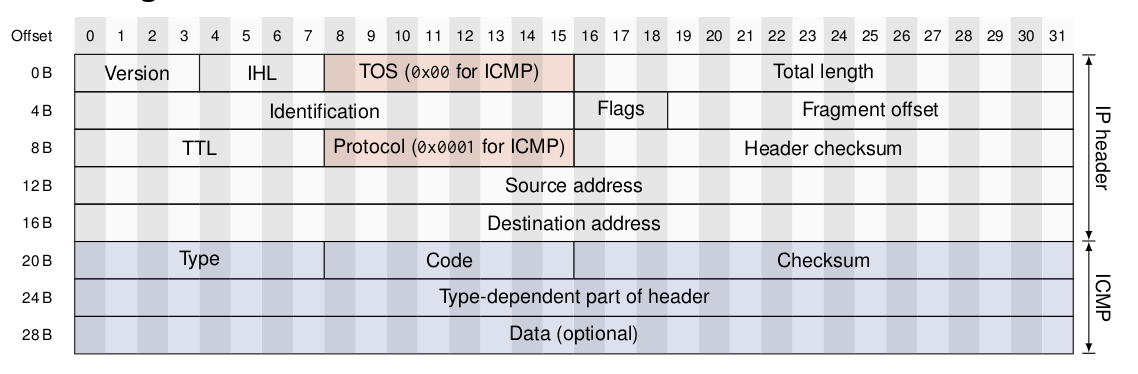
\includegraphics[width=.8\textwidth]{figures/icmp_message.png}
  \caption{ICMP Message}\label{fig:icmp_message}
\end{figure}

\subsection{Active Network Measurements}
Network is actively measured by several parties like network providers (to manage traffic or reduce cost), service providers (to adjust service, get information about clients, \dots), clients (to check services, get best one) or researchers (for performance evaluation of algorithms).
Furthermore malicious traffic can be detected.
\vspace{5pt}

Measurements are done with probe packets and looking at the packet loss, one-way delay, RTTs or packet inter-arrival times.

\subsubsection*{(Paris-) Traceroute}
Traceroute uses different TTLs in the IP header to get the route from the source to the destination.
In case of load balancing though, traceroute might fail due to the appearance of ghost paths when successive packets are routed on different routes.

Load balancing routers usually use the IP-5-Tuple to determine routes, so to fix this Paris traceroute uses different fields than normal traceroute (e.g.\ destination port for tcp) to do measurements.

\subsection{Address Resolution Protocol (ARP)}
ARP is used to map IP addresses to MAC addresses.
For that, an ARP broadcast is sent by the sender of an IP packet to get the MAC address of the next hop.
The node with the specified IP address responds and the sender caches the mapping and is able to send the resulting Ethernet frame.
In case we have a network with routers, the router then again does an ARP request for the IP address specified in the received IP header and so the procedure begins again at that point.
Cached information times out when not refreshed within a certain time threshold.
\begin{figure}[H]
  \centering
  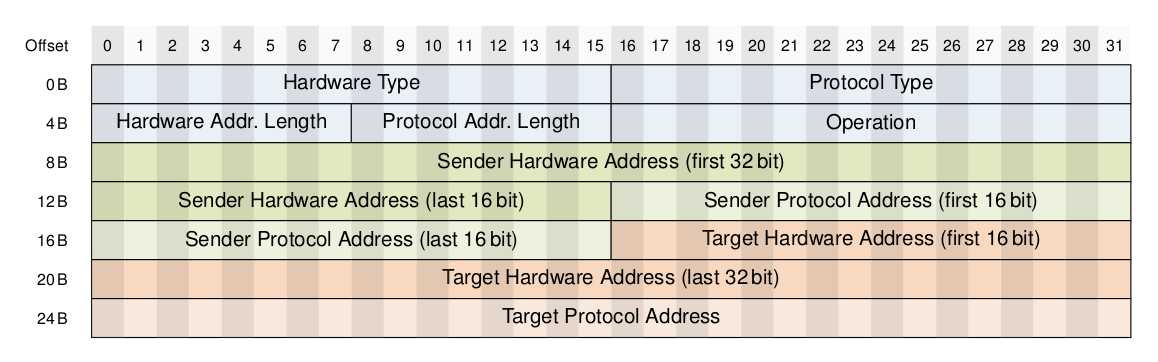
\includegraphics[width=.8\textwidth]{figures/arp_packet.png}
  \caption{ARP Packet}\label{fig:arp_packet}
\end{figure}

\textbf{Reverse ARP} also exists, but is rarely used.

\textbf{Proxy ARP} also responds for ARP request of one of its networks with ARP responses for hosts of another network.
This enables transparent subnet gatewaying (two LANs with in same subnet), a host joining LAN via VPN (VPN server does proxy ARP) and to include host that are separated via firewalls (firewall handles proxy ARP).
\vspace{5pt}

Since ARP is stateless and not authenticated, ARP responses can easily be forged to poison the cache of hots which can be used to redirect traffic.

\subsection{Routing}
Routers are layer 3 devices that maintain forwarding tables, implement routing protocols and forward IP packets based on the forwarding table and the destination IP address.

\textbf{Routing} is the process on the control plane, where the forwarding table an hence the path incoming packets will follow is calculated.
\textbf{Forwarding} then is the actual directing of packets to an outgoing link according to the previously calculated forwarding table.
